\documentclass[10pt,a4paper,titlepage]{article}
\usepackage[utf8]{inputenc}
\usepackage{amsmath}
\usepackage{amsfonts}
\usepackage{amssymb}
\usepackage[ngerman]{babel}
\usepackage[pdftex]{graphicx}
\usepackage[vmargin=3cm, hmargin=2cm]{geometry}
\usepackage{tabularx}

\setlength{\parindent}{0pt}
\setlength{\parskip}{2pt}

\title{Entwurfsdokument}
\author{Simon Bischof \and Jan Haag \and Adrian Herrmann \and Lin Jin \and Tobias Schlumberger \and Matthias Schnetz}

\makeindex

\begin{document}

\thispagestyle {empty}
\vspace*{4cm}
\begin{center}
\begin {huge}
Entwurfsdokument\\
\end{huge}
Simon Bischof, Jan Haag, Adrian Herrmann, Lin Jin, Tobias Schlumberger, Matthias Schnetz\\
\vspace{3cm}
\begin{huge}
Praxis der Softwareentwicklung \\
Projekt 3:\\
Automatisches Pr\"{u}fen der Korrektheit von Programmen\\
Gruppe 1\\
\vspace{2cm}

\includegraphics[height=2cm]{images/Logo.pdf}\\[0.5cm]
\end{huge}
\begin{huge}
WS 2011/2012
\end{huge}
\end{center}
\newpage
\tableofcontents
\newpage

\section{Klassendiagramme}
\subsection{"Ubersicht}
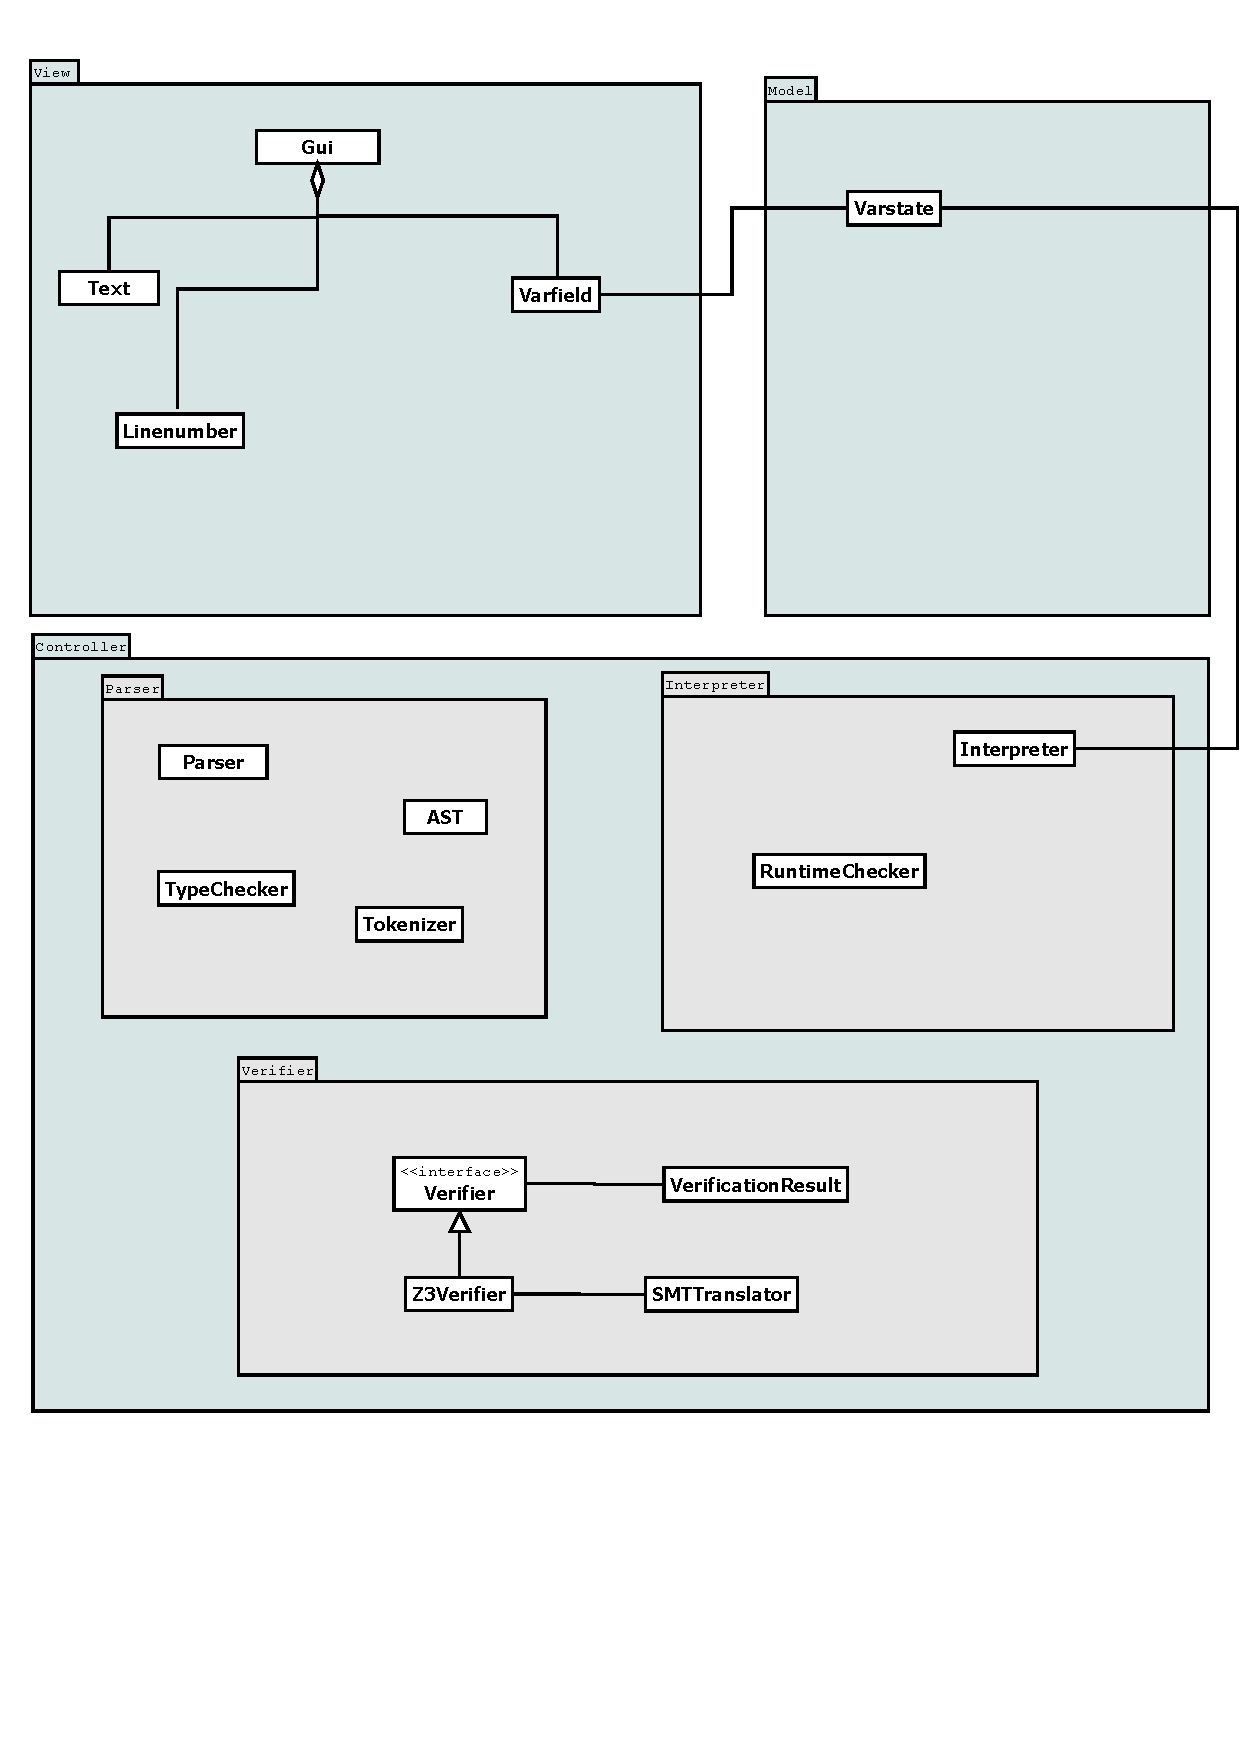
\includegraphics[scale=0.8]{images/ClassOverview.pdf}
\subsection{Feinstruktur der Komponenten}
\subsubsection{Parser}
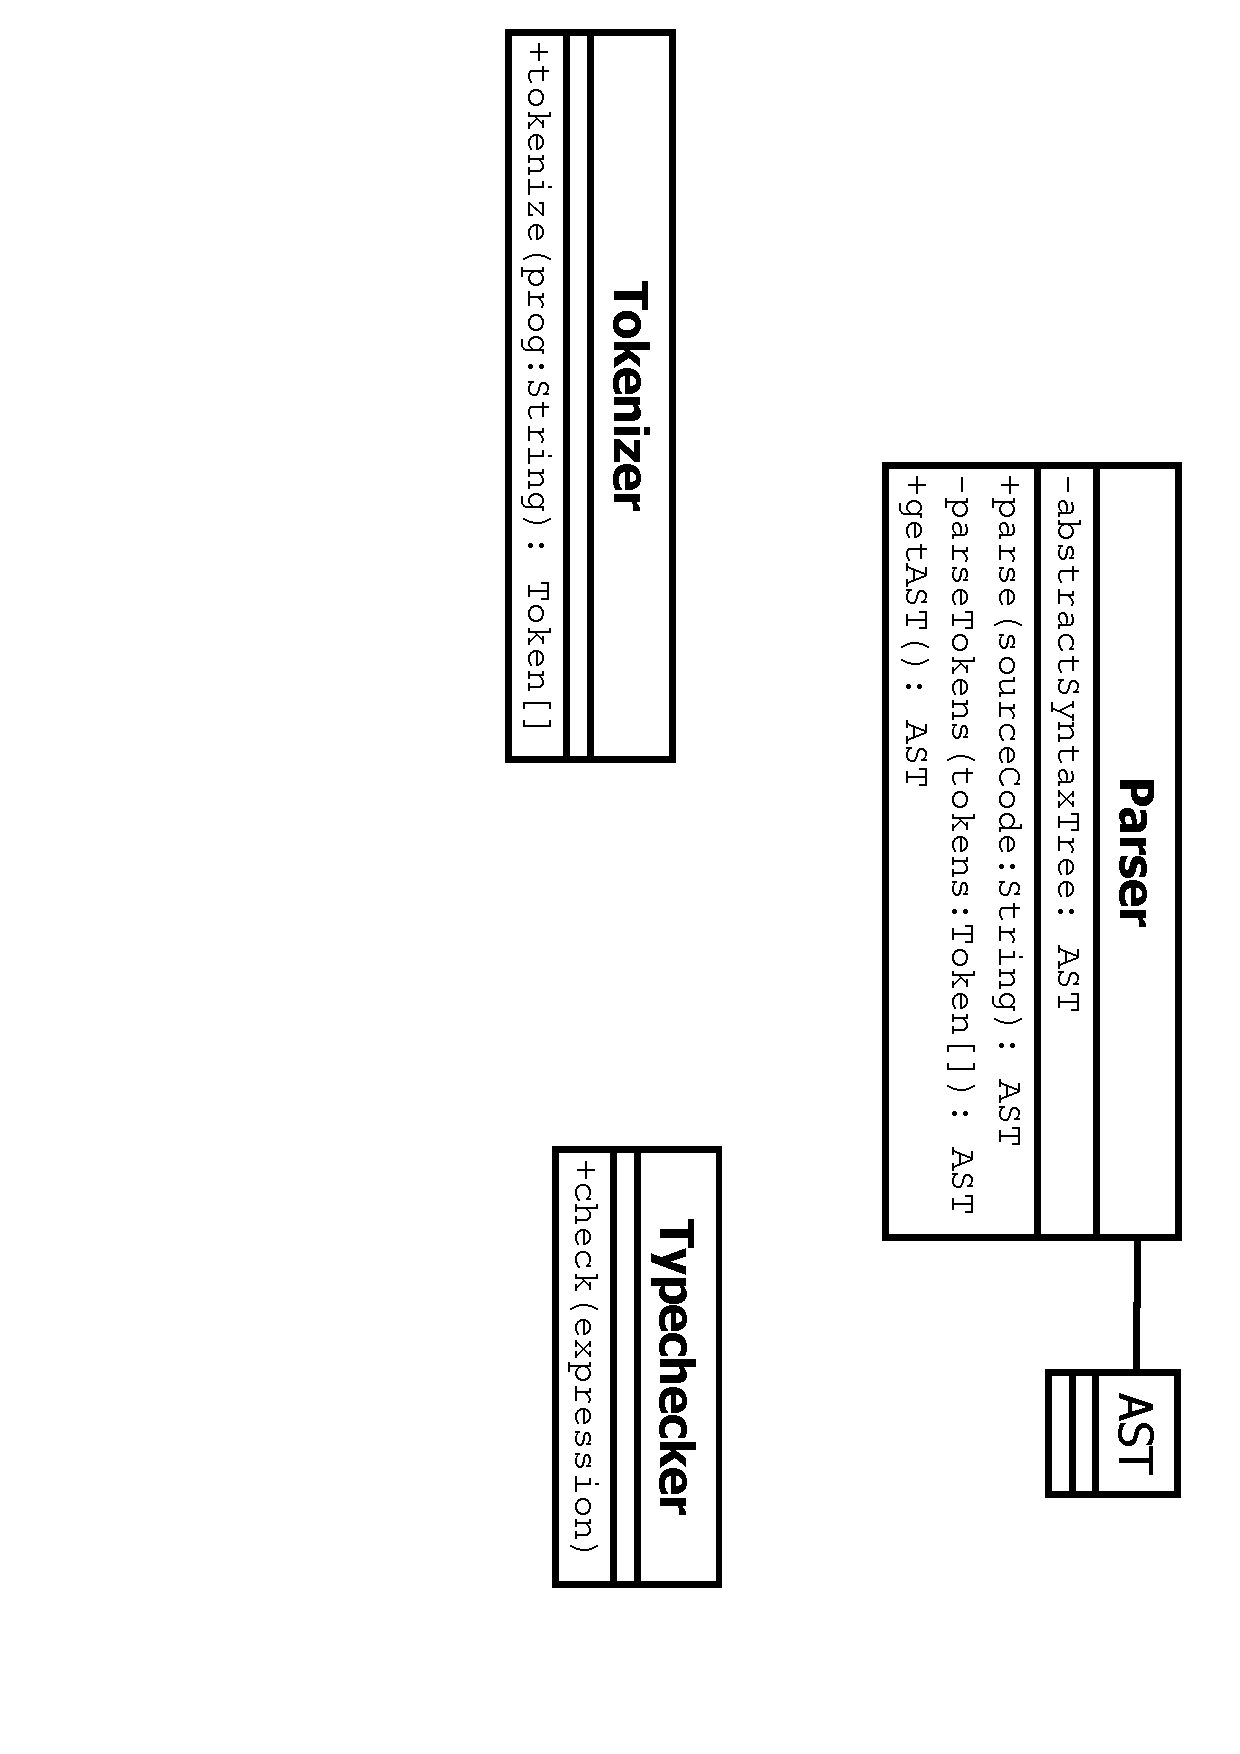
\includegraphics[angle=90, scale=0.6]{images/ClassParser.pdf}
\subsubsection{Interpreter}
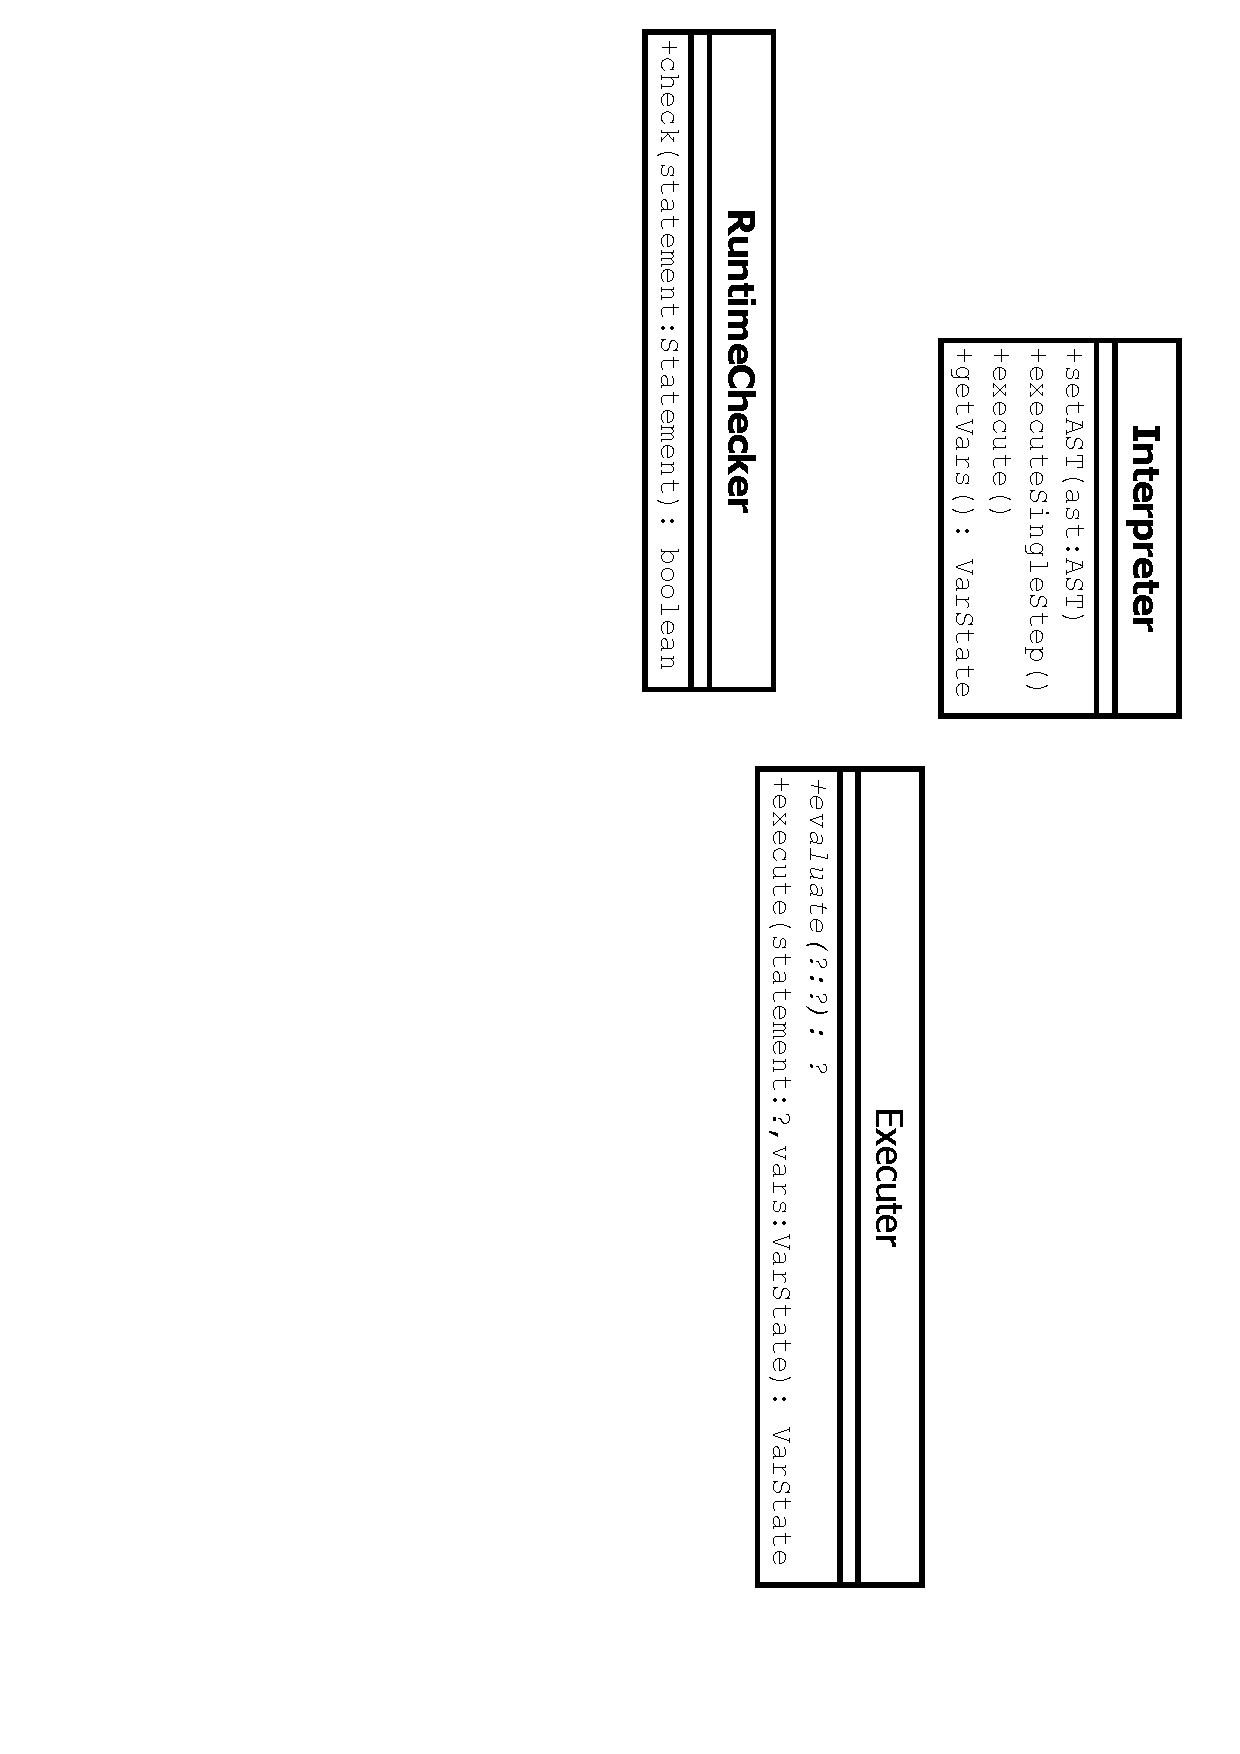
\includegraphics[angle=90, scale=0.6]{images/ClassInterpreter.pdf}
\subsubsection{Beweiser}
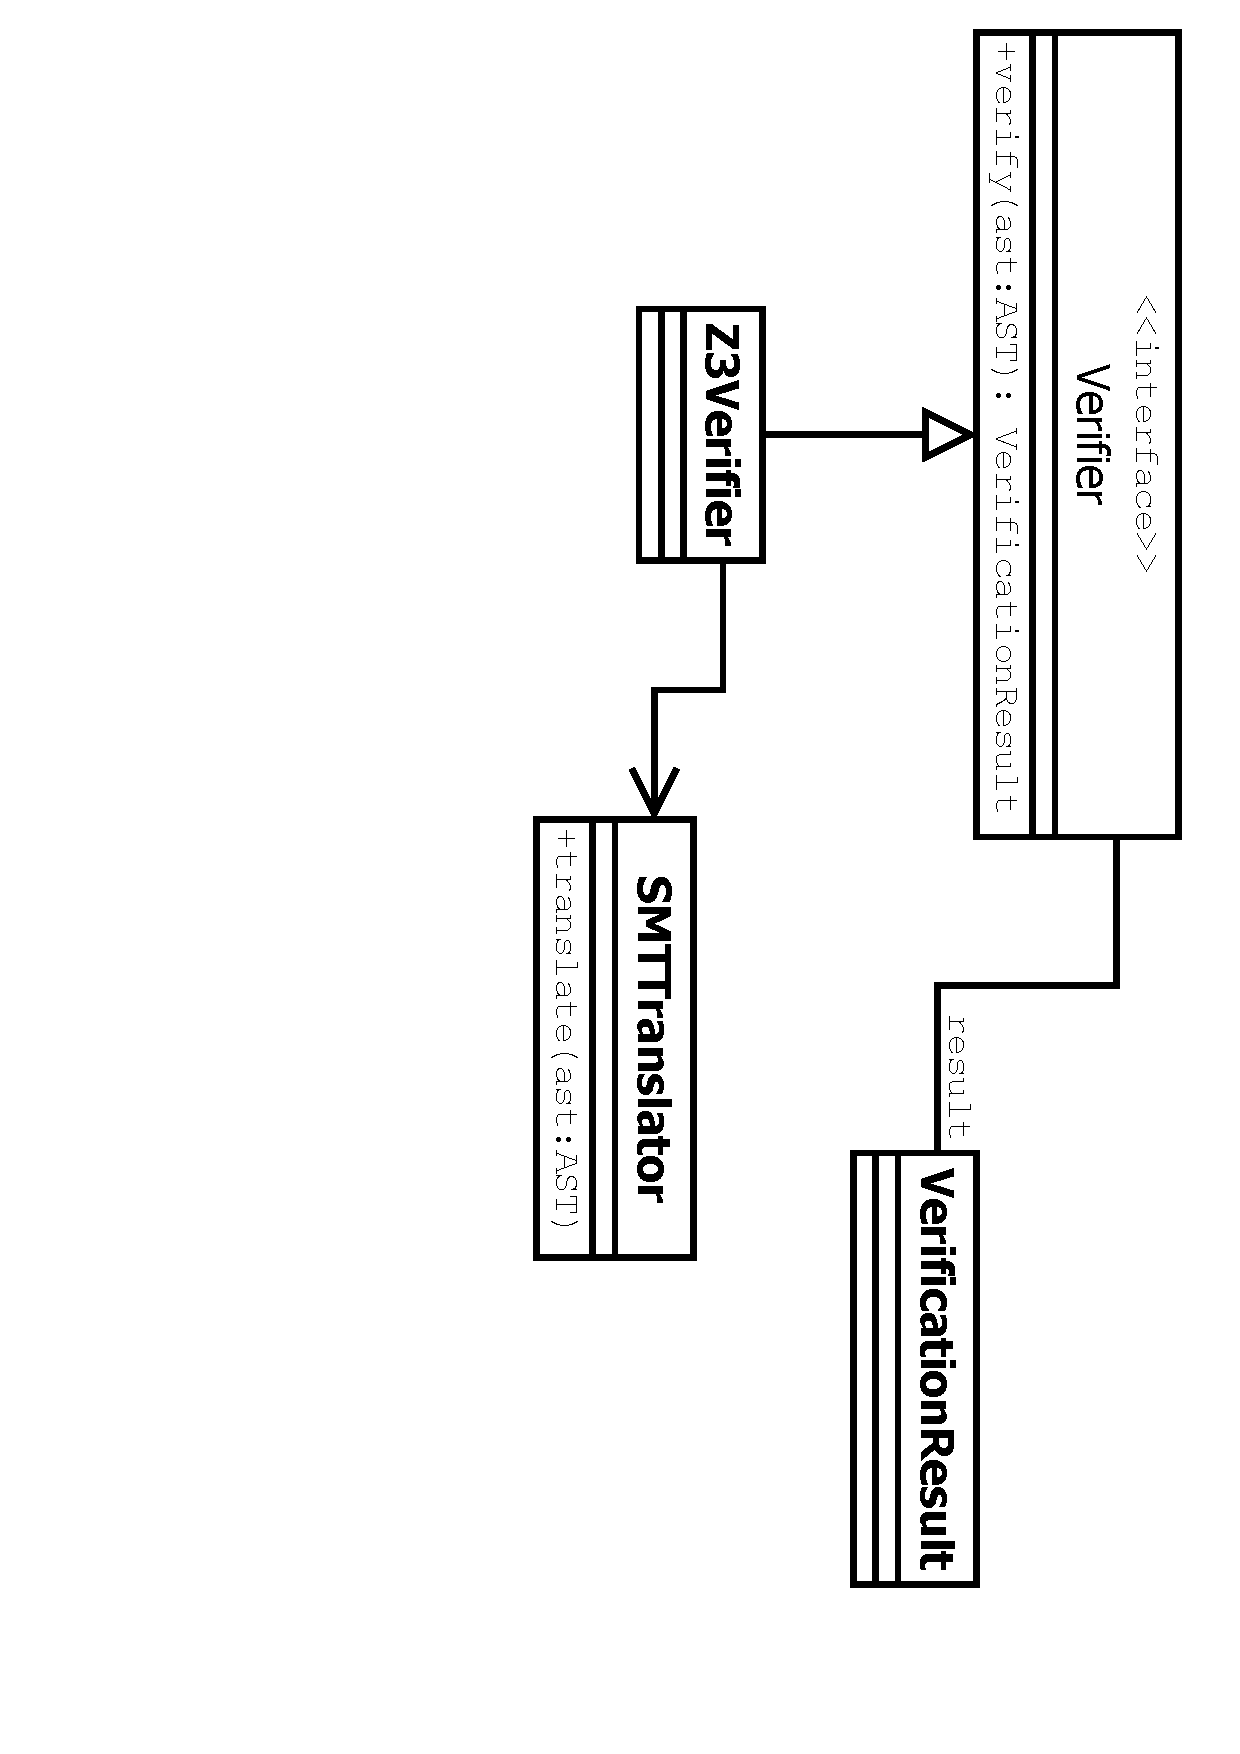
\includegraphics[angle=90, scale=0.6]{images/ClassVerifier.pdf}
\subsubsection{GUI}
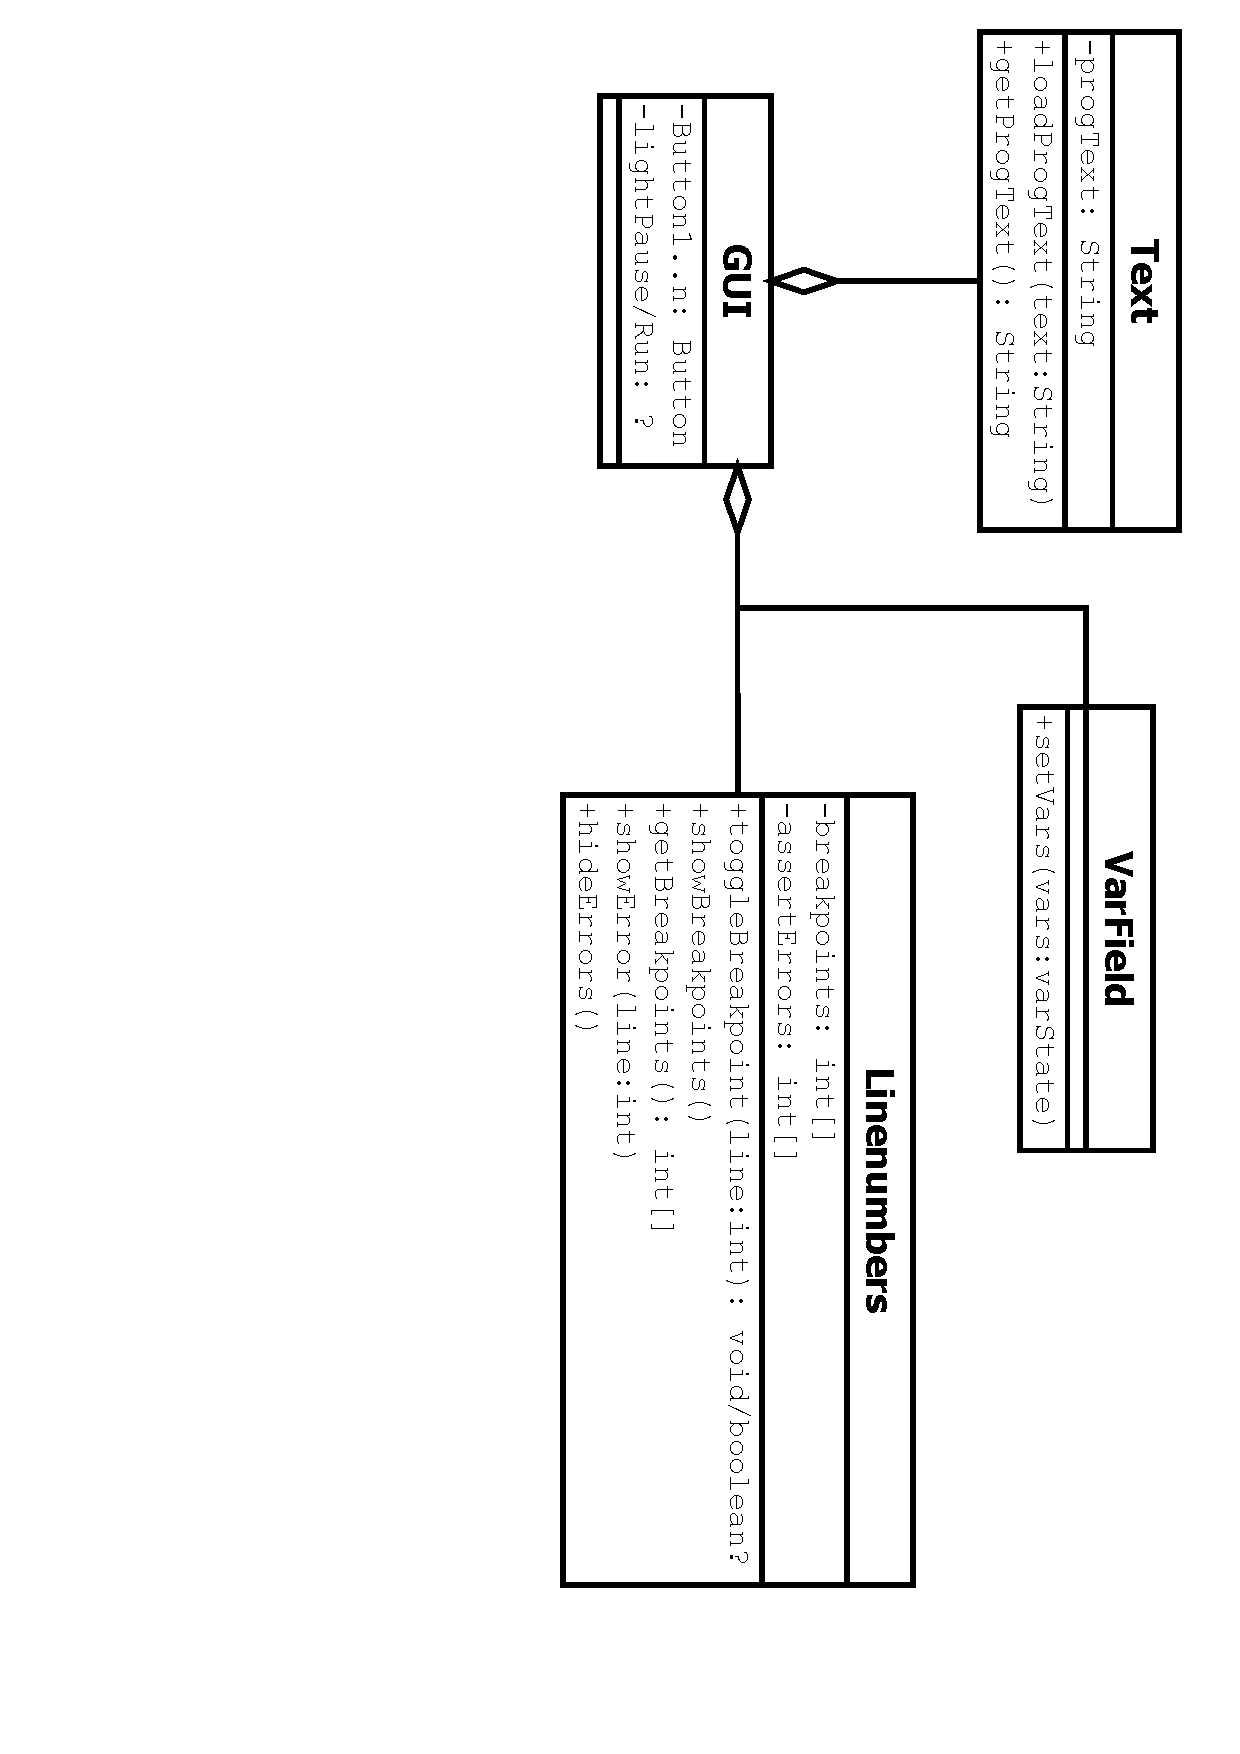
\includegraphics[angle=90, scale=0.6]{images/ClassGui.pdf}

\section{Verhaltensdiagramme}
\subsection{Aktivit"atsdiagramme}
\subsubsection{Parser/Type-Checker}
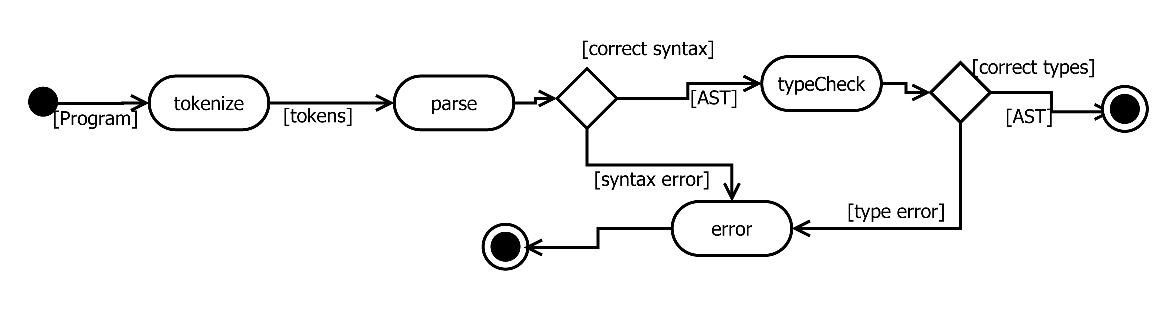
\includegraphics[angle=90, scale=0.45]{images/AktivitaetParser.pdf}
\subsection{Zustandsdiagramm}
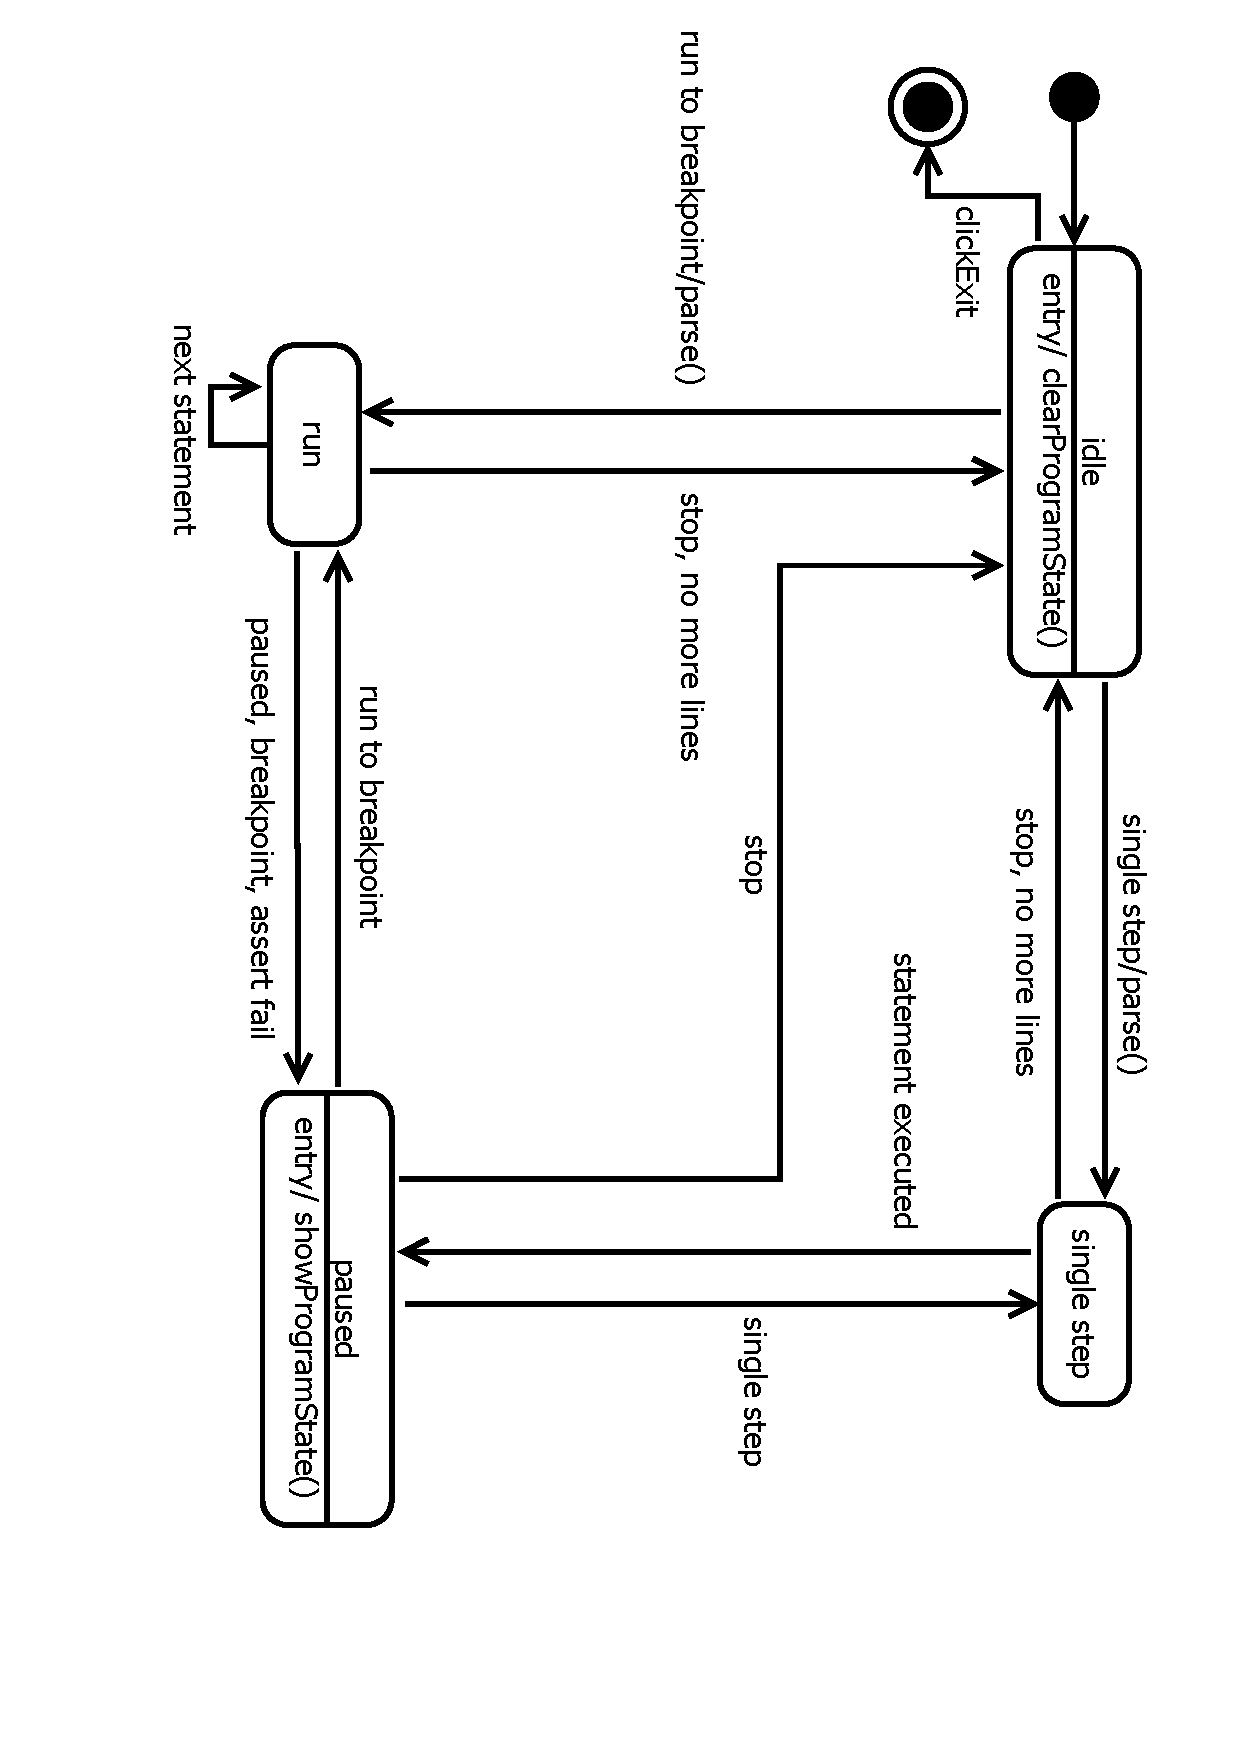
\includegraphics[angle=90, scale=0.6]{images/Zustandsdiagramm.pdf}

\newpage

\section{Syntax der While-Sprache}
\subsection{"Ubersicht der Schl"usselw"orter und Sonderzeichen}
\begin{ttfamily}
\begin{tabular}{| l  l |}
\hline
\hspace*{1cm}boolean & $\to$ type\_specifier\hspace*{2cm}\\\hline
\hspace*{1cm}else & $\to$ if\_statement\hspace*{2cm}\\\hline
\hspace*{1cm}false & $\to$ logical\_expression\\\hline
\hspace*{1cm}if & $\to$ if\_statement\\\hline
\hspace*{1cm}int & $\to$ type\_specifier\\\hline
\hspace*{1cm}return & $\to$ statement\\\hline
\hspace*{1cm}true & $\to$ logical\_expression\\\hline
\hspace*{1cm}while & $\to$ while\_statement\\\hline
\hspace*{1cm}0..9 & $\to$ integer\_literal\\\hline
\hspace*{1cm}a..z,A..Z,\_\hspace*{0.5cm} & $\to$ identifier\\\hline
\hspace*{1cm}\& & $\to$ logical\_expression\\\hline
\hspace*{1cm}| & $\to$ logical\_expression\\\hline
\hspace*{1cm}! & $\to$ logical\_expression\\\hline
\hspace*{1cm}!= & $\to$ testing\_expression\\\hline
\hspace*{1cm}== & $\to$ testing\_expression\\\hline
\hspace*{1cm}< & $\to$ testing\_expression\\\hline
\hspace*{1cm}<= & $\to$ testing\_expression\\\hline
\hspace*{1cm}> & $\to$ testing\_expression\\\hline
\hspace*{1cm}>= & $\to$ testing\_expression\\\hline
\hspace*{1cm}+ & $\to$ numeric\_expression\\\hline
\hspace*{1cm}- & $\to$ numeric\_expression\\\hline
\hspace*{1cm}* & $\to$ numeric\_expression\\\hline
\hspace*{1cm}/ & $\to$ numeric\_expression\\\hline
\hspace*{1cm}\% & $\to$ numeric\_expression\\\hline
\hspace*{1cm}, & $\to$ arglist \\
 & $\to$ parameter\_list \\
 & $\to$ variable\_declaration \\
 & $\to$ variable\_initializer\\\hline
\hspace*{1cm}; & $\to$ statement \\
 & $\to$ variable\_declaration\\\hline
\hspace*{1cm}= & $\to$ variable\_declarator\\\hline
\hspace*{1cm}( & $\to$ expression \\
 & $\to$ if\_statement \\
 & $\to$ methode\_declaration \\
 & $\to$ while\_statement\\\hline
\hspace*{1cm}) & $\to$ expression \\
 & $\to$ if\_statement \\
 & $\to$ methode\_declaration \hspace*{5cm}\\
 & $\to$ while\_statement\\\hline
\hspace*{1cm}[ & $\to$ expression \\
 & $\to$ type \\\hline
\hspace*{1cm}] & $\to$ expression \\
 & $\to$ type \\\hline
\hspace*{1cm}\{ & $\to$ statement\_block \\
 & $\to$ variable\_initializer\\\hline
\hspace*{1cm}\} & $\to$ statement\_block \\
 & $\to$ variable\_initializer\\\hline
\hspace*{1cm}\# & $\to$ comment\\\hline
\end{tabular}
\end{ttfamily}

\subsection{Startsymbol}
\texttt{compilation\_unit}
\subsection{Produktionsregeln}
\begin{ttfamily}
\shorthandoff{"}
arglist ::=  expression \{ "," expression \}\\

comment ::= "\#" "... text ..."\\

compilation\_unit ::= \{ field\_declaration \}\\

expression ::= numeric\_expression \\
		\hspace*{3cm}$\mid$ testing\_expression\\
		\hspace*{3cm}$\mid$ literal\_expression\\
		\hspace*{3cm}$\mid$ logical\_expression\\
		\hspace*{3cm}$\mid$ identifier\\
		\hspace*{3cm}$\mid$ ( "(" expression ")" )\\
		\hspace*{3cm}$\mid$ ( expression ( ( "(" $[$ arglist $]$ ")" )\\
					\hspace*{6.3cm}$\mid$ ( "[" expression "]" ) ) )\\
					
field\_declaration ::= ( $[$ comment $]$ ( method\_declaration \\
					\hspace*{7cm}$\mid$ variable\_declaration ) )\\

identifier ::= "a..z,A..Z,\_" \{ "a..z,A..Z,\_,0..9" \}\\

if\_statement ::= "if" "(" expression ")" statement\_block $[$ "else" statement\_block $]$\\

integer\_literal ::= ( "0..9" \{ "0..9" \} )\\

literal\_expression ::= integer\_literal\\

logical\_expression ::= ( "!" expression )\\
		\hspace*{4.5cm}$\mid$ ( expression ( "\&" \\
				\hspace*{7.5cm}$\mid$ "|" \\
				\hspace*{7.5cm}$\mid$ ( "\&" "\&" )\\ 
				\hspace*{7.5cm}$\mid$ ( "|" "|" ) ) expression )\\
		\hspace*{4.5cm}$\mid$ "true" \\
		\hspace*{4.5cm}$\mid$ "false" \\
		
method\_declaration ::= type identifier "(" $[$ parameter\_list $]$ ")" ( statement\_block )\\

numeric\_expression ::= ( ( "+" \\
			\hspace*{5.3cm}$\mid$ "-" ) expression ) \\
			\hspace*{4.5cm}$\mid$ ( expression ( "+" \\
				\hspace*{7.7cm}$\mid$ "-" \\
				\hspace*{7.7cm}$\mid$ "*" \\
				\hspace*{7.7cm}$\mid$ "/" \\
				\hspace*{7.7cm}$\mid$ "\%" ) expression ) \\
								
parameter ::= type identifier \\

parameter\_list ::= parameter \{ "," parameter \} \\

statement ::= variable\_declaration \\
		\hspace*{3cm}$\mid$ ( expression ";" ) \\
		\hspace*{3cm}$\mid$ ( statement\_block ) \\
		\hspace*{3cm}$\mid$ ( if\_statement ) \\
		\hspace*{3cm}$\mid$ ( while\_statement ) \\
		\hspace*{3cm}$\mid$ ( "return" $[$ expression $]$ ";" ) \\
		\hspace*{3cm}$\mid$ ( ";" ) \\
		
statement\_block ::= "\{" \{ statement \} "\}" \\

testing\_expression ::= ( expression ( ">" \\
					\hspace*{7cm}$\mid$ "<" \\
					\hspace*{7cm}$\mid$ ">=" \\
					\hspace*{7cm}$\mid$ "<=" \\
					\hspace*{7cm}$\mid$ "==" \\
					\hspace*{7cm}$\mid$ "!=" ) expression ) \\

type ::= type\_specifier \{ "[" "]" \} \\

type\_specifier ::= "boolean" \\
		\hspace*{3.8cm}$\mid$ "int" \\

variable\_declaration ::= type variable\_declarator \{ "," variable\_declarator \} ";" \\

variable\_declarator ::= identifier $[$ "=" variable\_initializer $]$ \\

variable\_initializer ::= expression \\
		\hspace*{4.8cm}$\mid$ ( "\{" $[$ variable\_initializer \{ "," variable\_initializer \} $]$ "\}" ) \\

while\_statement ::= "while" "(" expression ")" statement\_block \\
\shorthandon{"}
\end{ttfamily}

\end{document}

